\section{Benchmark operation}
% \addcontentsline{toc}{section}{Benchmark operation}

     \paragraph*{}
     In this section, we will discuss the operator used in the benchmarks: General Matrix 
     Multiplication (GEMM) operation.
     \par

     \paragraph*{}
     General Matrix Multiplication (GEMM) is the operation $C = AB + C$, where $A$ and $B$ are input matrices, 
     and $C$ is a pre-existing matrix overwritten by the result. For matrices of sizes 
     $M \times K$ (A), $K \times N$ (B), and $M \times N$ (C), the product of $A$ and $B$ results in 
     $M \times N$ values, each derived from a dot product of $K$ elements. The total number of fused 
     multiply-add operations (FMAs) required is $M \times N \times K$, and since each FMA consists of 
     both a multiplication and an addition, the total number of floating-point operations (FLOPs) is 
     $2 \times M \times N \times K$.
     \par

     \paragraph*{}
     To particularize the expression for theoretical time, we substitute the sequence of operations factor $S$ with 4, 
     which corresponds to the four sequences of operations required for matrix multiplication:
     \begin{enumerate} 
          \item Accessing values in matrix A. 
          \item Accessing values in matrix B. 
          \item Performing the multiplication. 
          \item Storing the results in matrix C. 
     \end{enumerate}
     \par



\subsection{Dot product function}
% \addcontentsline{toc}{subsection}{Dot product function}
The first step toward evaluating the speed of our CPU is to ensure that we are using optimized operators: this means that the 
operator, in this case the dot product, is able to utilize all available hardware resources and does not waste them. To achieve 
this, the dot product operator included by Julia (\texttt{matrix\_multiplication}) is compared with a function that would perform the dot 
product in the most basic way (\texttt{my\_matrix\_multiplication}):

\vspace*{0.5cm}

\lstinputlisting[language=Julia]{code/1-efficiency_dot_product/dot_func_comparison-v2.jl}

\vspace*{1cm}

\begin{figure}[h]
    \begin{center}
        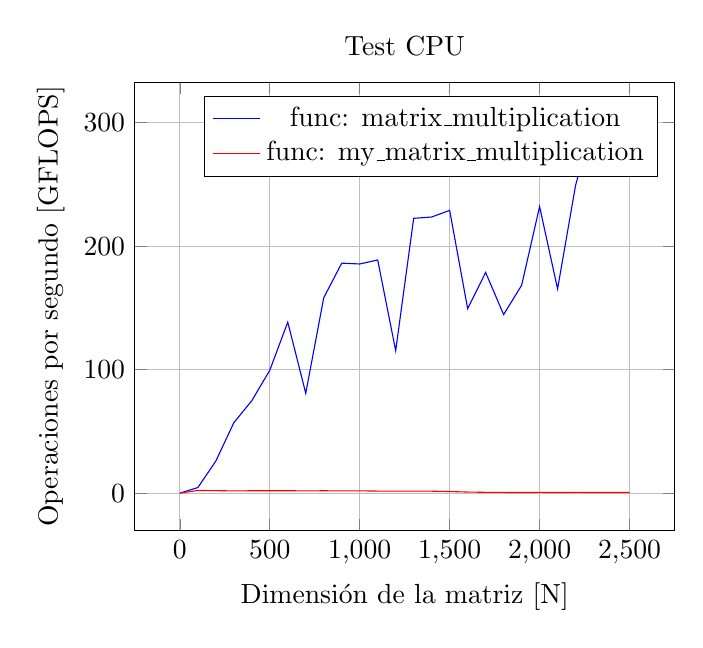
\begin{tikzpicture}
\begin{axis}[
    xlabel={Dimensión de la matriz [N]}, 
    ylabel={Operaciones por segundo [GFLOPS]}, 
    title={Test CPU}, 
    grid=major, 
    legend entries={func: matrix\_multiplication, func: my\_matrix\_multiplication},
    legend pos=north east
]
    \addplot[no marks, blue]
        table[row sep={\\}]
        {
            \\
            0.0  0.0  \\
            100.0  4.505580161029435  \\
            200.0  25.90157724416931  \\
            300.0  56.99491162094584  \\
            400.0  74.81460006920351  \\
            500.0  99.47991898355397  \\
            600.0  138.45150960218908  \\
            700.0  80.841705929692  \\
            800.0  158.1745422090465  \\
            900.0  186.1970516501426  \\
            1000.0  185.5222344223705  \\
            1100.0  188.76211619492446  \\
            1200.0  115.30743578149881  \\
            1300.0  222.4895517508976  \\
            1400.0  223.541866911042  \\
            1500.0  228.9426519346536  \\
            1600.0  149.35724605074793  \\
            1700.0  178.65956741256764  \\
            1800.0  144.57104491846164  \\
            1900.0  168.24198834607196  \\
            2000.0  231.9644286028204  \\
            2100.0  165.38387166340138  \\
            2200.0  249.1662040723394  \\
            2300.0  302.4547056863648  \\
            2400.0  293.0968504237342  \\
            2500.0  285.9051147985887  \\
        }
        ;
    \addplot[no marks, red]
        table[row sep={\\}]
        {
            \\
            0.0  0.0  \\
            100.0  2.1552235074538406  \\
            200.0  2.012742927064109  \\
            300.0  1.8100606792675045  \\
            400.0  1.9166144538963483  \\
            500.0  1.9504521187020196  \\
            600.0  1.956153046806178  \\
            700.0  1.808849811943694  \\
            800.0  1.9157676621337185  \\
            900.0  1.8033434276574258  \\
            1000.0  1.8490797457392572  \\
            1100.0  1.6770770087976277  \\
            1200.0  1.6745879627741946  \\
            1300.0  1.5897517669006394  \\
            1400.0  1.5775137097949514  \\
            1500.0  1.2917936425260046  \\
            1600.0  0.8788243783145658  \\
            1700.0  0.6600846997308975  \\
            1800.0  0.5669557178921565  \\
            1900.0  0.5093183521071399  \\
            2000.0  0.5692738621547873  \\
            2100.0  0.5235806635720697  \\
            2200.0  0.5646710827025357  \\
            2300.0  0.5501647945196996  \\
            2400.0  0.5477864813457809  \\
            2500.0  0.5470489285626592  \\
        }
        ;
\end{axis}
\end{tikzpicture}

   \end{center}
   \caption{Eficiencia del producto de matrices, probado en una CPU 1,7 GHz Intel Core i7 de 4 núcleos}
   \label{}
\end{figure}



%!!! NOTE !!! For including .tex files that makes some graphics from a .jl file, use this:
% \begin{tikzpicture}
% \begin{axis}[xlabel={x}, ylabel={y}, title={Gráfico de ejemplo}]
%    \addplot[no marks]
%       table[row sep={\\}]
%       {
%           .
%           .
%           .
%        }
%       ;
% \end{axis}
% \end{tikzpicture}
\clearpage
\newpage